% =====================================================================
%  Graduation Thesis
%  School of Engineering, Tohoku University
%  Department of Mechanical and Aerospace Engineering (IMAC)
%
%  Formatted to the departmental submission specification:
%    - A4, portrait, horizontal writing, two-sided, left-side binding
%    - Margins: top 20 mm, bottom 25 mm, binding (inner) 25 mm,
%               fore-edge (outer) 25 mm
%    - Page number centred in the bottom margin
%    - Figures placed inline in the body text
%    - No CV / curriculum vitae section
%
%  Build:  latexmk -pdf graduation_thesis.tex
%     or:  pdflatex -> biber -> pdflatex -> pdflatex
%  The separate spine sheet for binding is in spine.tex.
% =====================================================================

\documentclass[12pt, a4paper, twoside, openright]{report}

% --------------------------- Encoding & fonts ------------------------
\usepackage[utf8]{inputenc}
\usepackage[T1]{fontenc}
\usepackage{amsmath, amssymb}       % must precede newtxmath (\Bbbk clash)
\usepackage{newtxtext, newtxmath}   % Times New Roman-compatible text + math
\usepackage{microtype}

% --------------------------- Core packages ---------------------------
\usepackage{graphicx}
\usepackage{booktabs}
\usepackage{multirow}
\usepackage{siunitx}
\usepackage{float}
\usepackage{enumitem}
\usepackage{caption}
\usepackage{subcaption}
\usepackage{setspace}
\usepackage{fancyhdr}
\usepackage{emptypage}              % suppress headers/footers on blank versos
\usepackage[hidelinks]{hyperref}
% Citation style: IEEE numeric, i.e. bracketed [1] in the text, with the
% reference list ordered by first citation. This is the convention used across
% mechanical and aerospace engineering, and the department does not mandate an
% alternative. To switch to APA author-date instead, install biblatex-apa and
% replace the line below with:
%     \usepackage{csquotes}
%     \usepackage[backend=biber, style=apa]{biblatex}
% No other change is needed; the \cite commands in the body are style-agnostic.
\usepackage[backend=biber, style=ieee, sorting=none]{biblatex}

\graphicspath{{figures/}{figures/photos/}{../analysis/results/}}
\addbibresource{references.bib}

% Permit line breaks inside URLs/DOIs in the bibliography
\setcounter{biburllcpenalty}{7000}
\setcounter{biburlucpenalty}{8000}

% --------------------------- Page geometry ---------------------------
% Departmental spec: top 20 mm, bottom 25 mm, binding 25 mm, fore-edge 25 mm.
% `bindingoffset` is 0 because the binding allowance is already the full
% 25 mm inner margin required by the spec.
\usepackage[
    a4paper,
    top=20mm,
    bottom=25mm,
    inner=25mm,
    outer=25mm,
    footskip=12mm,      % keeps the page number inside the 25 mm bottom margin
    headsep=6mm
]{geometry}

\onehalfspacing

% Give TeX some slack on lines containing unbreakable \texttt{} file paths
\emergencystretch=3em

% --------------------- Headers and footers ---------------------------
% Page number centred in the bottom margin on every page, per the spec.
\pagestyle{fancy}
\fancyhf{}
\fancyfoot[C]{\thepage}
\renewcommand{\headrulewidth}{0pt}
\renewcommand{\footrulewidth}{0pt}

\fancypagestyle{plain}{%          % chapter-opening pages
    \fancyhf{}%
    \fancyfoot[C]{\thepage}%
    \renewcommand{\headrulewidth}{0pt}%
}

% --------------------------- Captions --------------------------------
\captionsetup{font=small, labelfont=bf, width=0.9\textwidth}
\captionsetup[sub]{font=small, labelfont=bf}

% --------------------------- Convenience -----------------------------
\newcommand{\thesistitle}{Tactile-Feedback Teleoperation: Grip Force and Grasping Performance Across Haptic Actuator Types for Fragile and Deformable Objects}
\newcommand{\authorname}{Adriel, Santoso, Imaran}
\newcommand{\studentid}{C2TB1701}          % TODO: insert actual student ID
\newcommand{\labname}{Hashimoto Laboratory}
\newcommand{\supervisorname}{Prof.\ Koichi Hashimoto}
\newcommand{\graduationdate}{September, 2026}

% Marks passages that are still placeholders in this draft.
\newcommand{\todo}[1]{\textit{[TODO: #1]}}

\begin{document}

% =====================================================================
%  COVER PAGE  (per the departmental cover sample)
% =====================================================================
\begin{titlepage}
    \centering
    \thispagestyle{empty}
    \singlespacing

    \vspace*{25mm}

    {\fontsize{18}{22}\selectfont Graduation Thesis\par}
    \vspace{6mm}
    {\fontsize{18}{22}\selectfont School of Engineering, Tohoku University\par}

    \vspace{40mm}

    {\fontsize{20}{26}\selectfont\bfseries \thesistitle \par}

    \vspace{40mm}

    {\fontsize{18}{22}\selectfont Department of Mechanical and Aerospace Engineering\par}
    \vspace{4mm}
    {\fontsize{18}{22}\selectfont \labname\par}

    \vspace{20mm}

    {\fontsize{18}{22}\selectfont \studentid\quad \authorname\par}

    \vfill

    {\fontsize{18}{22}\selectfont (\graduationdate)\par}

    \vspace*{20mm}
\end{titlepage}

\cleardoublepage

% =====================================================================
%  FRONT MATTER
% =====================================================================
\pagenumbering{roman}
\setcounter{page}{1}

\chapter*{Abstract}
\addcontentsline{toc}{chapter}{Abstract}

Teleoperation cuts off the tactile signals that inform grip force in direct
grasping, so an operator must rely solely on vision to determine how hard a
remote gripper is squeezing. This becomes a problem with objects that show no
visual signs before breaking. This thesis implements tactile feedback to
complete the closed-loop haptic process and investigates whether tactile
feedback improves grasping of such objects, and whether the haptic actuator
used to deliver it matters.

The operator's thumb and index finger are tracked with markerless hand
tracking, and the resulting pinch aperture commands a Robotiq 2F-85 adaptive
gripper equipped with vision-based 9DTact tactile sensors at its fingertips.
Contact deformation is reduced in real time to a deformation-volume force
proxy and a normalised haptic intensity value, which is streamed back to a
wearable actuator array on the operator's hand, driven by an ESP32-C6. The
same pipeline renders two mechanically distinct actuator types: linear
resonant actuators (LRAs), driven by a bipolar resonant carrier whose envelope
encodes intensity, and electromagnetic (EM) bistable pin actuators, driven by
short latching H-bridge pulses.

Twenty-two participants took part in a study comparing three feedback
conditions (visual-only, LRA, and EM) while grasping fragile and deformable
objects. For fragile objects, both types of tactile feedback sharply cut down
on squeezing after the object was already fully grasped, and raised the
object's survival rate from 62\% with vision alone to 81\% with the LRA and
78\% with the EM. Deformable objects, which have no clear breaking point,
showed no consistent difference between conditions. Participants also
preferred both haptic conditions over vision alone and most often chose the
LRA as their favourite, though no single survey question reliably told the two
actuators apart.

These results show that tactile feedback clearly helps, but they do not show
which actuator helps more. A larger study, with counterbalanced condition
order, matched actuator placement, and a properly calibrated force
measurement, would be needed to rank the two actuator types with confidence.

\cleardoublepage

\tableofcontents
\cleardoublepage
\listoffigures
\cleardoublepage
\listoftables
\cleardoublepage

% =====================================================================
%  MAIN MATTER
% =====================================================================
\pagenumbering{arabic}
\setcounter{page}{1}

% =====================================================================
\chapter{Introduction}
\label{ch:introduction}
% =====================================================================

\section{Background and Motivation}
\label{sec:background}

Teleoperated robots are used wherever a human should not, or cannot, be
physically present: nuclear decommissioning, disaster response, minimally
invasive surgery, and the handling of hazardous or contaminated material. In
each case the operator issues motion commands through a master interface and
the robot reproduces them at the remote site, while sensory information about
the remote environment is returned through a feedback channel \cite{zheng2024,huang2019}. The quality of
that feedback channel bounds what the operator can safely do.

In practice the feedback channel is almost always visual. A camera stream tells
the operator where the gripper is and, sometimes, whether it has closed on the
object. What it does not convey is \emph{how hard} the gripper is squeezing.
Human grasping normally regulates force through cutaneous mechanoreceptors in
the fingertips, which report the onset of contact, the distribution of pressure,
and incipient slip within tens of milliseconds. When that channel is removed,
grip force is controlled open-loop, by guesswork, and the guess is
systematically conservative in the wrong direction: operators squeeze harder
than necessary because the cost of dropping an object is immediate and visible
whereas the cost of over-squeezing is not \cite{huang2019}.

For rigid, robust objects this matters little. It matters a great deal for
fragile objects, which fail abruptly beyond a force threshold, and for
deformable objects, which yield progressively without a clear failure point,
because in both cases the visual signature of impending failure either arrives
too late to act on or does not exist until the failure itself.

\section{The Role of Touch in Human Grasping}
\label{sec:role-of-touch}

Precision grasping in humans is not a single act of closing the fingers but a
continuous control loop. On contact, fast-adapting afferents signal the
transition from free motion to loaded contact; slowly-adapting afferents then
encode the sustained normal force; and micro-slip events, detected before gross
slip occurs, drive rapid reflexive increases in grip force \cite{johansson2009}. The result is a grip
that sits just above the minimum required to prevent slip, with a small safety
margin, and that adapts within a fraction of a second when the load changes.

Two features of this loop are relevant to the design of an artificial
substitute. First, the information that matters most is \emph{change}: contact
onset, slip onset, and force increments, rather than absolute force magnitude.
Second, the loop is closed continuously rather than sampled at discrete
decision points. Any haptic display that hopes to restore grip-force regulation
must therefore deliver a signal that is both temporally prompt and continuously
available, not a discrete alarm that fires once a threshold is crossed.

\section{Existing Haptic Feedback Approaches and Their Limitations}
\label{sec:existing-approaches}

Wearable haptic devices for the fingertip and hand fall broadly into three
families. \emph{Kinaesthetic} devices, such as exoskeletons and
force-reflecting master arms \cite{kuchenbecker_2010}, apply forces to the
finger joints and can in principle reproduce grip force directly, but they are
bulky, expensive, and constrain the operator's free motion.
\emph{Skin-deformation} devices, meaning normal-indentation and shear tactors,
apply displacement to the fingerpad and reproduce contact more faithfully than
vibration, but require comparatively large, slow actuators.
\emph{Vibrotactile} devices, including eccentric rotating-mass motors, linear
resonant actuators, and piezoelectric benders, are small, cheap, and fast, and
dominate practical deployments \cite{pacchierotti2017,choi2013}, but they render force \emph{indirectly}: they
substitute a vibration whose amplitude or frequency stands in for a force the
skin never actually feels.

Two gaps recur across this literature. First, most user studies evaluate a
single actuator against a no-feedback baseline, establishing that feedback helps
without establishing which kind of feedback helps most \cite{luo2024,abdi2020}; comparisons that hold
the sensing pipeline fixed and vary only the actuator are rare. Second, the
sensing side is frequently simplified: feedback is derived from motor current,
from a single load cell, or from a simulated contact model rather than from a
tactile sensor that actually measures the contact geometry.

\section{Tactile Sensing on the Robot Side}
\label{sec:tactile-sensing}

Vision-based tactile sensors resolve the second gap. A camera images the inner
surface of a deformable elastomer pad; when the pad contacts an object, the
resulting deformation field is reconstructed from the image, giving a dense
depth map of the contact patch at camera frame rate \cite{donggelsight2021,dahiya2010}. The 9DTact sensor used in
this work belongs to this family \cite{lin2023} and is compact enough to mount on a
conventional two-finger gripper without redesigning the finger.

Such a sensor supplies far more information than a haptic display of the kind
described above can render: a full depth map versus, typically, one scalar per
finger. Bridging that gap requires an explicit reduction, a mapping from
contact geometry to actuator drive, and the choice of reduction is itself a
design decision that this thesis makes explicit and holds constant across the
conditions being compared.

\section{Problem Statement}
\label{sec:problem-statement}

This thesis addresses a compound question that the literature has generally
split in two:

\begin{enumerate}[label=(\roman*)]
    \item Does tactile feedback, derived from a real vision-based tactile sensor
          and rendered on a wearable actuator array, measurably improve
          grip-force regulation and grasp outcomes when a teleoperator handles
          fragile and deformable objects, relative to a visual-only baseline?
    \item Given the same sensing and intensity-computation pipeline, does the
          \emph{type} of actuator used to render the signal, a continuously
          modulated resonant vibrator versus a discretely latching
          electromagnetic pin, change those outcomes?
\end{enumerate}

The second question is the one this work is structured to answer, because it
requires a system in which everything upstream of the actuator can be held
identical while the actuator itself is exchanged.

\section{Objectives}
\label{sec:objectives}

\begin{enumerate}
    \item Integrate vision-based tactile sensing into a Robotiq 2F-85 adaptive
          gripper and derive a real-time contact-intensity signal from it.
    \item Design and build a five-channel wearable actuator array, driven by an
          ESP32-C6, that can render that signal through either LRA or EM
          bistable pin actuators without any change upstream of the driver.
    \item Command the gripper from the operator's own pinch aperture using
          markerless hand tracking, so that the operator's control effort is
          comparable across conditions.
    \item Run a within-subjects user study comparing visual-only, LRA, and EM
          feedback on fragile and deformable objects, collecting both
          per-tick quantitative logs and per-condition subjective ratings.
    \item Analyse the resulting data to answer the two questions of
          Section~\ref{sec:problem-statement}, and state explicitly which
          confounds limit the strength of the answer.
\end{enumerate}

\section{Contributions}
\label{sec:contributions}

The specific contributions of this thesis are:

\begin{itemize}
    \item An end-to-end open teleoperation stack, covering tactile sensing,
          hand tracking, gripper control, the serial haptic link, and firmware,
          in which the haptic actuator is the only component that changes between
          experimental conditions.
    \item An intensity-rendering scheme for bistable electromagnetic pin
          actuators that approximates a sustained, graded sensation through
          burst-and-gap pulsing, permitting a like-for-like comparison against
          a continuously modulated LRA.
    \item An $N=22$ within-subjects study quantifying the effect of tactile
          feedback and of actuator type on grip-force regulation and object
          survival for fragile and deformable objects.
    \item A metric, \emph{excess deformation}, that isolates the force applied
          after the tactile display has saturated, and therefore after further
          squeezing conveys no new information to the operator.
\end{itemize}

\section{Thesis Structure}
\label{sec:structure}

Chapter~\ref{ch:literature} reviews robotic grasping with force feedback,
vision-based tactile sensing, and wearable haptic actuation, and identifies the
comparative gap this work addresses. Chapter~\ref{ch:system} describes the
system architecture: the sensing pipeline, the hand-tracking control mapping,
the serial link, and the two actuator drive circuits.
Chapter~\ref{ch:methodology} specifies the user study: participants, design,
task, materials, protocol, and instruments. Chapter~\ref{ch:results} reports the
quantitative and subjective results. Chapter~\ref{ch:discussion} interprets
them, sets out the limitations, and connects the system to energy-based models
of the teleoperation loop. Chapter~\ref{ch:conclusion} concludes and states the
future work that follows most directly from the findings.

% =====================================================================
\chapter{Literature Review}
\label{ch:literature}
% =====================================================================

\section{Robotic Grasping and Force Feedback}
\label{sec:lit-grasping}

\todo{Expand to 2--3 paragraphs. Cover: force-controlled grasping of unknown
    objects; grip-force/load-force coupling in teleoperation; evidence that
    force-feedback reduces peak grasp force in bilateral systems; why current-based
    force estimation on an underactuated gripper is a proxy rather than a
    measurement.}

Starting points: \cite{zheng2024,huang2019,robotiq_manual}.

\section{Vision-Based Tactile Sensing}
\label{sec:lit-vbts}

\todo{Expand. GelSight lineage; photometric-stereo versus depth-from-shading
    reconstruction; the 9DTact design and its calibration procedure; what quantities
    (depth map, deformation volume, 6D force estimate) such sensors expose and at
    what latency.}

Starting points: \cite{donggelsight2021,lin2023,dahiya2010}.

\section{Tactile Sensing for Slip Detection and Manipulation}
\label{sec:lit-slip}

\todo{Expand. Incipient-slip detection from tactile imagery; closed-loop grasp
    force control driven by tactile signals; why a purely autonomous controller is
    not a substitute for operator-in-the-loop feedback in the fragile-object case.}

Starting points: \cite{taylor2021,garciarobledo2011,vipins2025}.

\section{Haptic Feedback in Teleoperation}
\label{sec:lit-haptics}

\todo{Expand. Taxonomy of wearable fingertip haptics; sensory substitution
    versus sensory restoration; evidence on vibrotactile feedback reducing grip
    force in prosthetics and teleoperation; typical study sizes ($N=10$--$12$) and
    effect sizes.}

Starting points: \cite{pacchierotti2017,pacchierotti2015,pacchierotti2015b,tsetserukou2010,luo2024,abdi2020}.

\section{Linear Resonant Actuators}
\label{sec:lit-lra}

\todo{Expand. Mass-spring resonant construction; narrow-band efficiency around
    resonance; amplitude modulation versus envelope (on-fraction) modulation;
    mechanical ring-up and ring-down time constants and their perceptual
    consequences.}

Starting points: \cite{verrillo1985,choi2013,pacchierotti2015}.

\section{Electromagnetic Bistable Pin Actuators}
\label{sec:lit-em}

\todo{Expand. The TacTiles dual-mode design; magnetic latching and zero
    holding-power operation; rendering continuous contact versus discrete spatial
    patterns; power and driver requirements relative to an LRA.}

Starting points: \cite{vechev2019}.

\section{The Comparative Gap}
\label{sec:lit-gap}

Across the work reviewed above, two observations motivate this thesis. Studies
that compare feedback modalities usually vary the actuator \emph{and} the
sensing or control pipeline at the same time, so an observed difference cannot
be attributed to the actuator. Studies that hold the pipeline fixed usually
evaluate a single actuator against no feedback at all. Consequently there is
little direct evidence on whether a continuously modulated vibrotactile display
and a discretely latching skin-contact display, driven from the same tactile
signal and the same intensity mapping, produce different grip-force regulation.
This thesis is constructed to supply exactly that comparison.

% =====================================================================
\chapter{System Architecture}
\label{ch:system}
% =====================================================================

\section{Overall Framework}
\label{sec:framework}

The system forms a single closed loop that begins and ends at the operator's
hand. The operator pinches; a camera tracks the pinch aperture; the aperture is
mapped to a commanded gripper opening; the gripper closes on the object; the
tactile sensors report the resulting contact deformation; the deformation is
reduced to a scalar intensity; and that intensity is rendered on the actuator
array worn on the operator's fingertips. Figure~\ref{fig:signalflow} shows the
signal path and the boundary between the host PC and the wearable hardware.

\begin{figure}[htbp]
    \centering
    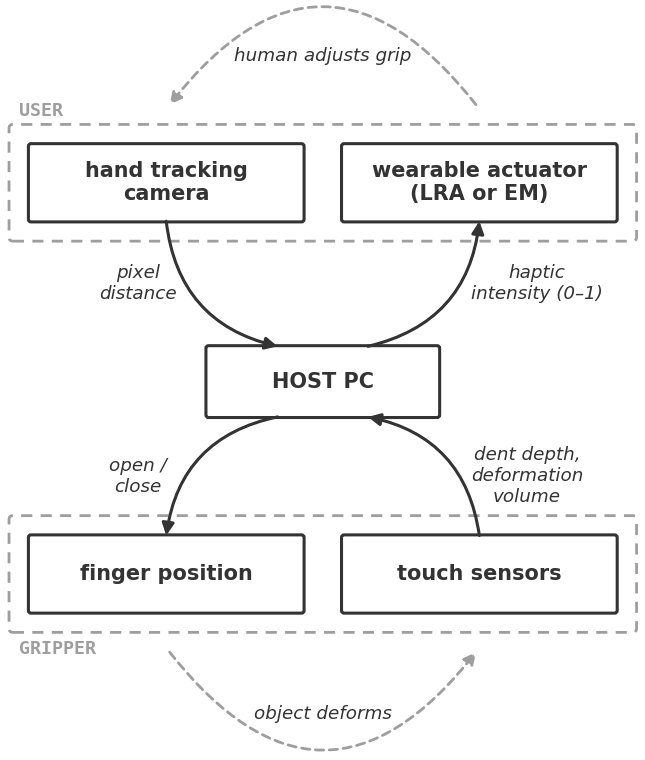
\includegraphics[width=0.85\textwidth]{preprint_fig1.png}
    \caption{Signal flow of the teleoperation loop. Everything upstream of the
        haptic driver is identical in the LRA and EM conditions; only the actuator
        and its drive stage differ.}
    \label{fig:signalflow}
\end{figure}

The loop runs at approximately \SI{30}{\hertz}, set by the tactile camera frame
rate, and is implemented as a set of cooperating threads on the host: a
tracking thread, a tactile-sensing thread, a gripper-command thread, and a
logging thread that writes one row per sensor update.

\begin{figure}[htbp]
    \centering
    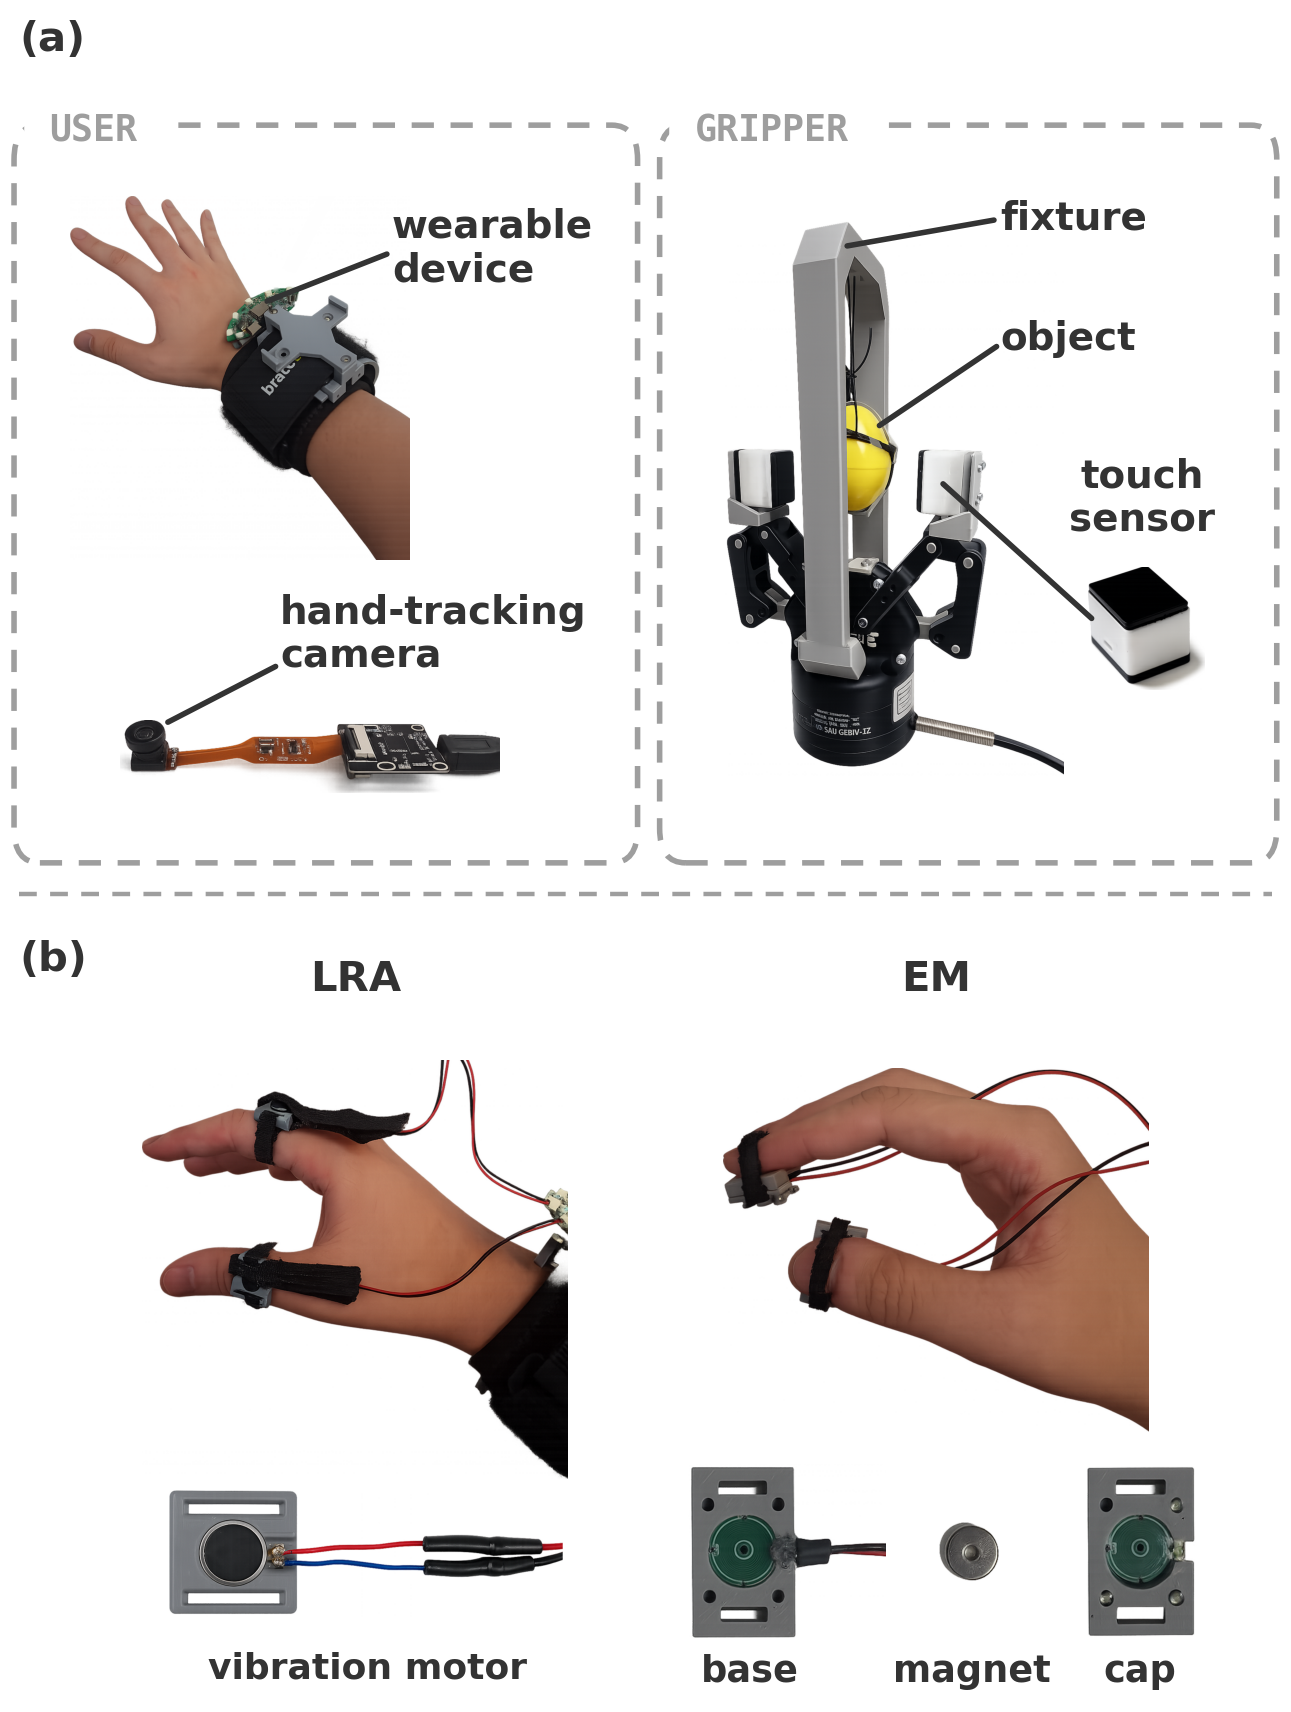
\includegraphics[width=0.9\textwidth]{preprint_fig2.png}
    \caption{Hardware. (a) The operator station and gripper apparatus, grouped
        as in Figure~\ref{fig:signalflow}. (b) The two actuator types compared in
        this study: LRA (left) and EM bistable pin (right).}
    \label{fig:hardware}
\end{figure}

\section{Operator-Side Control: Hand Tracking}
\label{sec:handtracking}

The gripper is commanded from the operator's own hand rather than from a
joystick or slider, so that the motor act of closing the gripper resembles the
motor act of closing the hand. A single RGB camera observes the operator's
dominant hand; a markerless hand-tracking model returns 2D landmark positions,
from which the thumb-tip to index-tip distance is computed each frame. This
pinch aperture is normalised against a per-participant calibration, taken from
a fully open and a fully closed pinch recorded at the start of the session, and
mapped linearly onto the gripper's commanded position register.

\todo{Add the calibration equation, the smoothing filter and its time constant,
    the dead-band used to suppress tracking jitter, and a note on the failure mode
    when the hand leaves the tracking volume.}

\section{Robotiq 2F-85 and Tactile Integration}
\label{sec:gripper}

The remote manipulator is a Robotiq 2F-85 adaptive two-finger gripper,
controlled from the host over Modbus RTU \cite{robotiq_manual}. The gripper exposes commanded
position, measured position, and motor current; the last of these is used as a
secondary, coarse indicator of grasp effort but is not the primary force proxy
in this study.

\subsection{Sensor Mounting}
\label{subsec:sensormount}

A 9DTact vision-based tactile sensor replaces the fingertip pad on the gripper
finger. The sensor comprises a deformable elastomer layer, a diffuse
illumination ring, and a camera imaging the inner surface of the layer.

\todo{Add the printed mount geometry, the standoff distance from camera to gel,
    cable routing, and a photograph of the assembled finger.}

\subsection{Calibration and Reconstruction}
\label{subsec:sensorcalib}

Calibration follows the 9DTact procedure \cite{lin2023}: a reference frame of the undeformed
gel is captured, then a ball of known radius is pressed into the gel at a set of
positions to fit the mapping from pixel intensity to indentation depth. From
this mapping, each incoming frame yields a depth map of the contact patch, from
which two quantities are derived:

\begin{itemize}
    \item \textbf{Deformation volume}: the integral of indentation depth over
          the contact patch, in arbitrary units (a.u.). This is the primary
          grip-force proxy used throughout the analysis. It is uncalibrated: it
          is monotonic in applied force but is not expressed in newtons.
    \item \textbf{Maximum indentation depth}: the peak of the depth map, in
          millimetres. This is the quantity mapped to haptic intensity.
\end{itemize}

\subsection{Depth-to-Intensity Mapping}
\label{subsec:mapping}

Maximum indentation depth $d$ is mapped to a normalised haptic intensity
$u \in [0,1]$ by clipping and linear scaling against a fixed ceiling
$d_{\max}$:
\begin{equation}
    u = \min\!\left(\frac{\max(d - d_0,\, 0)}{d_{\max} - d_0},\; 1\right),
    \label{eq:mapping}
\end{equation}
where $d_0$ is the no-contact noise floor established at calibration and
$d_{\max} = \SI{1.0}{\milli\metre}$ is a safety ceiling above which the gripper
is commanded to stop closing. Equation~\eqref{eq:mapping} is identical in both
haptic conditions; the conditions differ only in how $u$ is realised physically.

The saturation implied by Equation~\eqref{eq:mapping} has a direct experimental
consequence. Once $d$ reaches $d_{\max}$, the display stops changing, and any
further squeezing by the operator delivers no new information. Deformation
volume accumulated after that point is therefore, by construction, effort the
feedback channel could not have discouraged. This is the \emph{excess
    deformation} metric defined in Section~\ref{sec:metrics}.

\section{ESP32-C6 Haptic Driver}
\label{sec:driver}

Intensity values are streamed from the host to an ESP32-C6 over a USB serial
link as short binary packets, one per control tick. The firmware maintains the
commanded intensity for each of five channels and regenerates the corresponding
drive waveform locally, so a dropped packet degrades to a held value rather than
to silence.

\subsection{LRA Drive}
\label{subsec:lra-drive}

Each linear resonant actuator is driven differentially from an H-bridge with a
bipolar square-wave carrier at approximately \SI{200}{\hertz}. Intensity is
rendered by envelope modulation: within a fixed \SI{50}{\milli\second} window,
the carrier is gated on for a fraction of the window proportional to $u$.

This is a compromise rather than the ideal drive. An LRA's perceived amplitude
is properly modulated by varying the drive \emph{amplitude} at the actuator's
resonant frequency; the microcontroller's standard PWM peripheral cannot
generate the phase-locked antiphase pair that amplitude-modulated bipolar drive
would require. The consequence for interpretation is taken up in
Section~\ref{sec:limitations}.

\subsection{EM Bistable Pin Drive}
\label{subsec:em-drive}

Each electromagnetic actuator is a bistable pin that latches magnetically in
either the extended or retracted state and requires power only to switch between
them \cite{vechev2019}. A short H-bridge pulse of one polarity extends the pin against the
operator's fingerpad; a pulse of the opposite polarity retracts it.

Because a latched pin produces no ongoing sensation, a sustained, graded
percept is approximated by repeated pulsing: intensity $u$ is mapped to the
burst-to-gap ratio of an extend/retract pulse train, so that higher intensity
produces more frequent contact events per unit time.

\todo{Insert the schematic of the five-channel driver board, the H-bridge part
    number, supply voltage and current budget, and the measured pulse width required
    for reliable latching.}

\section{Data Logging}
\label{sec:logging-arch}

The host writes one CSV row per control tick for the duration of each recorded
trial, containing the timestamp, commanded and measured gripper position, motor
current, deformation volume, maximum indentation depth, the rendered haptic
intensity, and the active control mode. These logs are the sole source of the
quantitative metrics in Chapter~\ref{ch:results}.

% =====================================================================
\chapter{Experimental Methodology}
\label{ch:methodology}
% =====================================================================

\section{Participants}
\label{sec:participants}

Twenty-two participants ($N=22$) took part in the study. Eligibility required
normal or corrected-to-normal vision and no diagnosed sensory or motor
impairment affecting the dominant hand; a screening item recorded any such
impairment and was used to exclude affected responses from the subjective
analysis. Prior robotics or teleoperation experience was not required, and was
recorded as a covariate. All participants gave informed consent before taking
part.

The sample exceeds the $N=10$--$12$ typical of comparable vibrotactile
teleoperation studies, which was the target set during design; the larger sample
was recruited to improve power for the actuator-versus-actuator comparison,
which was expected a priori to have a smaller effect than the
feedback-versus-no-feedback comparison.

\section{Design and Counterbalancing}
\label{sec:design}

The study uses a within-subjects design with one factor, feedback condition, at
three levels: \textbf{visual-only} (V), \textbf{LRA}, and \textbf{EM}. Every
participant experienced all three conditions, which controls for individual
differences in manual dexterity and grip-force perception that would otherwise
dominate a between-subjects comparison at this sample size.

\todo{State the realised condition order explicitly. The presentation preprint
    records the order as fixed rather than counterbalanced; if that is correct, this
    section must say so plainly here and the resulting practice/fatigue confound
    must be carried into Section~\ref{sec:limitations} rather than described as
    controlled.}

Within each condition, participants performed five trials per object class,
giving ten trials per condition and thirty trials per participant, and 110
trials per condition per object class across the sample.

\section{Task and Materials}
\label{sec:task}

Participants sat at a workstation facing a display carrying the remote-view
camera feed, with no direct line of sight to the gripper. In the LRA and EM
conditions they wore the corresponding actuator array on the fingertips of the
dominant hand. The gripper stood vertically with its fingers pointing upward;
each object was presented in a fixed cradle at the end of a horizontal support
arm, positioned so that the object centre sat at a constant height of
\SI{16.5}{\centi\metre} aligned with the centre of the open finger gap. The
gripper body did not move during a trial: only the fingers opened and closed,
under hand-tracking control.

Each trial consisted of closing the gripper on the presented object, holding
briefly, and releasing it without dropping or visibly damaging it. Two object
classes were used, shown in Figure~\ref{fig:objects}:

\begin{itemize}
    \item \textbf{Fragile}: a hollow two-part plastic egg, which separates
          abruptly once the applied force exceeds the seam strength. Failure is
          discrete and unambiguous, and the object is replaced between trials.
    \item \textbf{Deformable}: a foam cube, which yields progressively and
          recovers between trials, with no discrete failure point.
\end{itemize}

\begin{figure}[htbp]
    \centering
    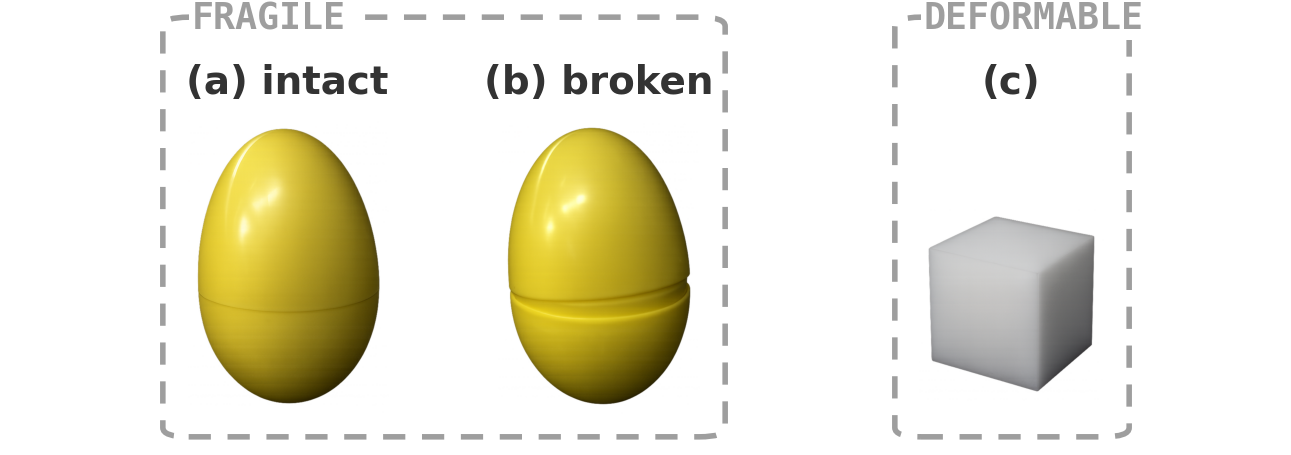
\includegraphics[width=0.85\textwidth]{preprint_fig4.png}
    \caption{Object classes. (a) The hollow plastic egg used as the fragile
        object. (b) The same egg with its halves separated, the failure event scored
        as breakage. (c) The foam cube used as the deformable object.}
    \label{fig:objects}
\end{figure}

\section{Session Protocol}
\label{sec:protocol}

Figure~\ref{fig:methodflow} summarises the session. Each session comprised:
(1) informed consent and task explanation; (2) per-participant pinch
calibration; (3) an untimed practice trial in each condition, in the order the
participant would encounter them, with no data recorded; (4) the three
experimental conditions, each completed in full before moving to the next;
(5) a post-condition questionnaire administered immediately after each
condition; and (6) a closing preference question and free-form interview.
Rest breaks were offered between conditions.

\begin{figure}[htbp]
    \centering
    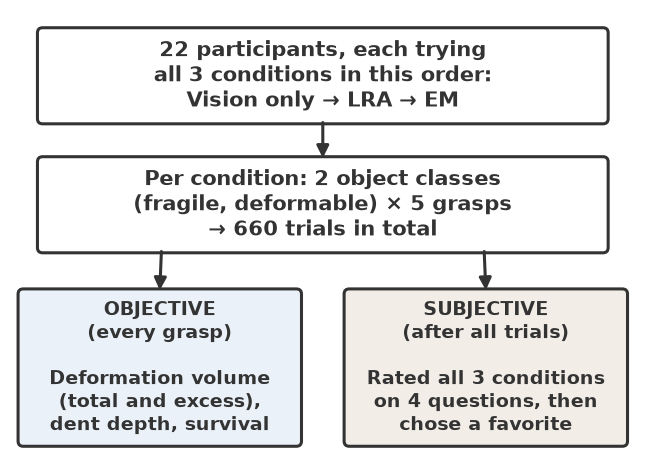
\includegraphics[width=0.8\textwidth]{preprint_fig3.png}
    \caption{Flowchart of the experimental session, $N=22$.}
    \label{fig:methodflow}
\end{figure}

\section{Instruments}
\label{sec:instruments}

\subsection{Quantitative Logging}
\label{subsec:logging}

Per-tick logs are as described in Section~\ref{sec:logging-arch}. Object
outcome, survived or broke, for fragile objects, was scored by the
experimenter immediately after each trial and recorded alongside the log.

\subsection{Post-Condition Questionnaire}
\label{subsec:questionnaire}

After each condition, participants rated a set of 7-point Likert items
(1 = strongly disagree, 7 = strongly agree) covering perceived force awareness,
contact detection, damage anticipation, mental effort, and sense of control.
Two further items, administered only in the LRA and EM conditions, addressed the
perceived responsiveness and naturalness of the feedback itself. A single
forced-choice preference question at the end of the session asked which
condition the participant would choose to perform the task again.

\todo{Reproduce the exact item wording as administered, in
    Appendix~\ref{app:questionnaire}, and confirm the item numbering used by the
    analysis pipeline matches it.}

\section{Analysis Procedures}
\label{sec:analysis-procedures}

Per-trial metrics (Section~\ref{sec:metrics}) are reduced to one value per
participant per condition per object class using the median across repeated
trials, so that a single unusually careless grasp cannot dominate a
participant's contribution. Cross-condition comparisons use the Friedman test,
the non-parametric repeated-measures analogue of one-way ANOVA, with pairwise
Wilcoxon signed-rank tests and Holm correction across the three condition pairs
where the omnibus test is significant. Fragile-object survival, being a paired
binary outcome, is tested with McNemar's test. Results are reported as medians
and interquartile ranges rather than means and standard deviations, for
robustness to the high-force outliers the study is designed to detect. All
analyses are implemented in the accompanying \texttt{analysis} package and
regenerate the tables and figures of Chapter~\ref{ch:results} from the raw logs.
CSV outputs referenced by filename in Chapter~\ref{ch:results} are written to
\texttt{analysis/results/}.

% =====================================================================
\chapter{Results}
\label{ch:results}
% =====================================================================

\section{Derived Per-Trial Metrics}
\label{sec:metrics}

Four metrics are computed from each trial log:

\begin{itemize}
    \item \textbf{Peak deformation volume} (a.u.): the maximum deformation
          volume reached during the trial; the primary grip-force proxy.
    \item \textbf{Excess deformation} (a.u.): deformation volume accumulated
          after maximum indentation depth has plateaued, i.e.\ after the haptic
          display has saturated per Equation~\eqref{eq:mapping} and further
          squeezing conveys nothing new.
    \item \textbf{Grip adjustments} (count): the number of squeeze/release
          reversals after the plateau, taken as a sign of searching for an
          appropriate grip rather than holding steady.
    \item \textbf{Peak indentation depth} (\si{\milli\metre}): the maximum of
          the depth map, reported mainly as a check on the safety ceiling.
\end{itemize}

\section{Fragile Objects}
\label{sec:results-fragile}

Table~\ref{tab:quant} summarises the fragile-object results.

\begin{table}[htbp]
    \centering
    \caption{Fragile-object results by condition (V = visual only). The first
        four rows give the median value for a participant, where lower is better.
        The last row is the percentage of all 110 trials per condition in which the
        object survived. Peak indentation depth differs little across conditions
        because the \SI{1.0}{\milli\metre} safety ceiling caps it before any
        difference could emerge.}
    \label{tab:quant}
    \begin{tabular}{@{}lrrr@{}}
        \toprule
                                       & V     & LRA   & EM    \\
        \midrule
        Peak deformation volume (a.u.) & 20100 & 12300 & 16000 \\
        Excess deformation (a.u.)      & 1530  & 170   & 260   \\
        Grip adjustments (\#)          & 7     & 5     & 2     \\
        Peak indentation depth (mm)    & 0.98  & 0.95  & 0.98  \\
        \midrule
        Objects surviving (\%)         & 62    & 81    & 78    \\
        \bottomrule
    \end{tabular}
\end{table}

Both haptic conditions reduced the force applied after the display had
saturated: median excess deformation fell roughly ninefold under the LRA and
roughly sixfold under the EM relative to visual-only feedback. Grip adjustments
fell most under the EM condition. Object survival rose from 62\% under
visual-only feedback to 81\% (LRA) and 78\% (EM), as shown in
Figure~\ref{fig:results}.

\begin{figure}[htbp]
    \centering
    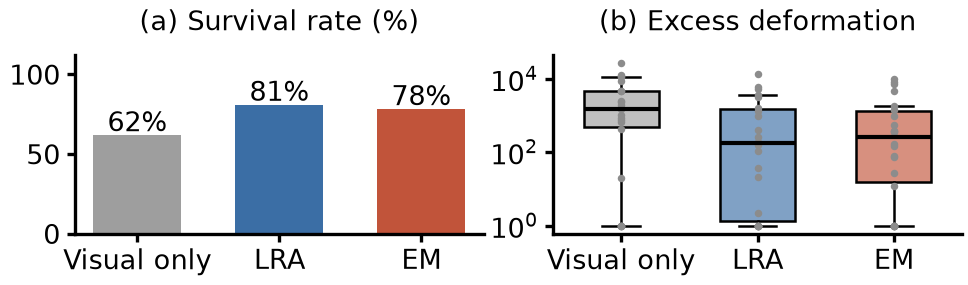
\includegraphics[width=0.9\textwidth]{preprint_fig5.png}
    \caption{Objective results for fragile objects. (a) Survival rate, 110
        trials per condition. (b) Excess deformation per participant (a.u.,
        $\log(x+1)$ scale).}
    \label{fig:results}
\end{figure}

\todo{Insert the omnibus Friedman statistics, the Holm-corrected pairwise
    $p$-values, and the McNemar result for survival, from the analysis outputs
    \texttt{section\_5\_3\_cross\_condition.csv} and
    \texttt{section\_5\_4\_fragile\_mcnemar.csv}. Report effect sizes alongside
    $p$-values.}

\section{Deformable Objects}
\label{sec:results-deformable}

Deformable objects showed no reliable difference between conditions on any of
the four metrics. This is consistent with the nature of the object class: a foam
cube has no failure threshold to avoid, so there is no penalty for squeezing
harder and correspondingly little for the feedback channel to correct.

\todo{Report the deformable-object table in the same format as
    Table~\ref{tab:quant}, together with the omnibus tests, so that the null result
    is stated with statistics rather than asserted.}

\section{Sensor-to-Actuator Latency}
\label{sec:latency}

\todo{Outstanding. The trial logs are timestamped at the control-loop rate
    ($\approx$\SI{30}{\hertz}) but do not establish true end-to-end latency from
    tactile frame capture to physical actuator motion. A bench measurement is
    required, combining a frame-capture timestamp, a serial packet timestamp, and
    either an oscilloscope or photodiode trigger on the actuator itself, reported
    once per
    actuator type as a latency distribution.}

\section{LRA Versus EM}
\label{sec:lra-vs-em}

Because the two haptic conditions share an identical sensing and
intensity-computation pipeline, a direct paired comparison between them isolates
the actuator-type variable. On the fragile-object metrics the two conditions
are close: the LRA yields the lower median excess deformation and the EM the
lower number of grip adjustments, and neither difference is large relative to
the spread across participants.

\todo{Insert the paired Wilcoxon results from
    \texttt{section\_5\_4\_lra\_vs\_em.csv} and the equivalence
    test from \texttt{section\_5\_9\_tost\_equivalence.csv}. If the TOST result
    supports equivalence within the chosen bound, say so explicitly: a null result
    and a demonstrated equivalence are different claims and should not be
    conflated.}

\section{Time-Series Behaviour}
\label{sec:timeseries}

Representative single-trial traces for each condition illustrate the behaviour
the excess-deformation metric is designed to capture: under visual-only
feedback, deformation volume continues to rise after indentation depth has
plateaued, whereas under both haptic conditions it tends to level off shortly
after the plateau.

\begin{figure}[htbp]
    \centering
    \begin{subfigure}[b]{0.48\textwidth}
        \centering
        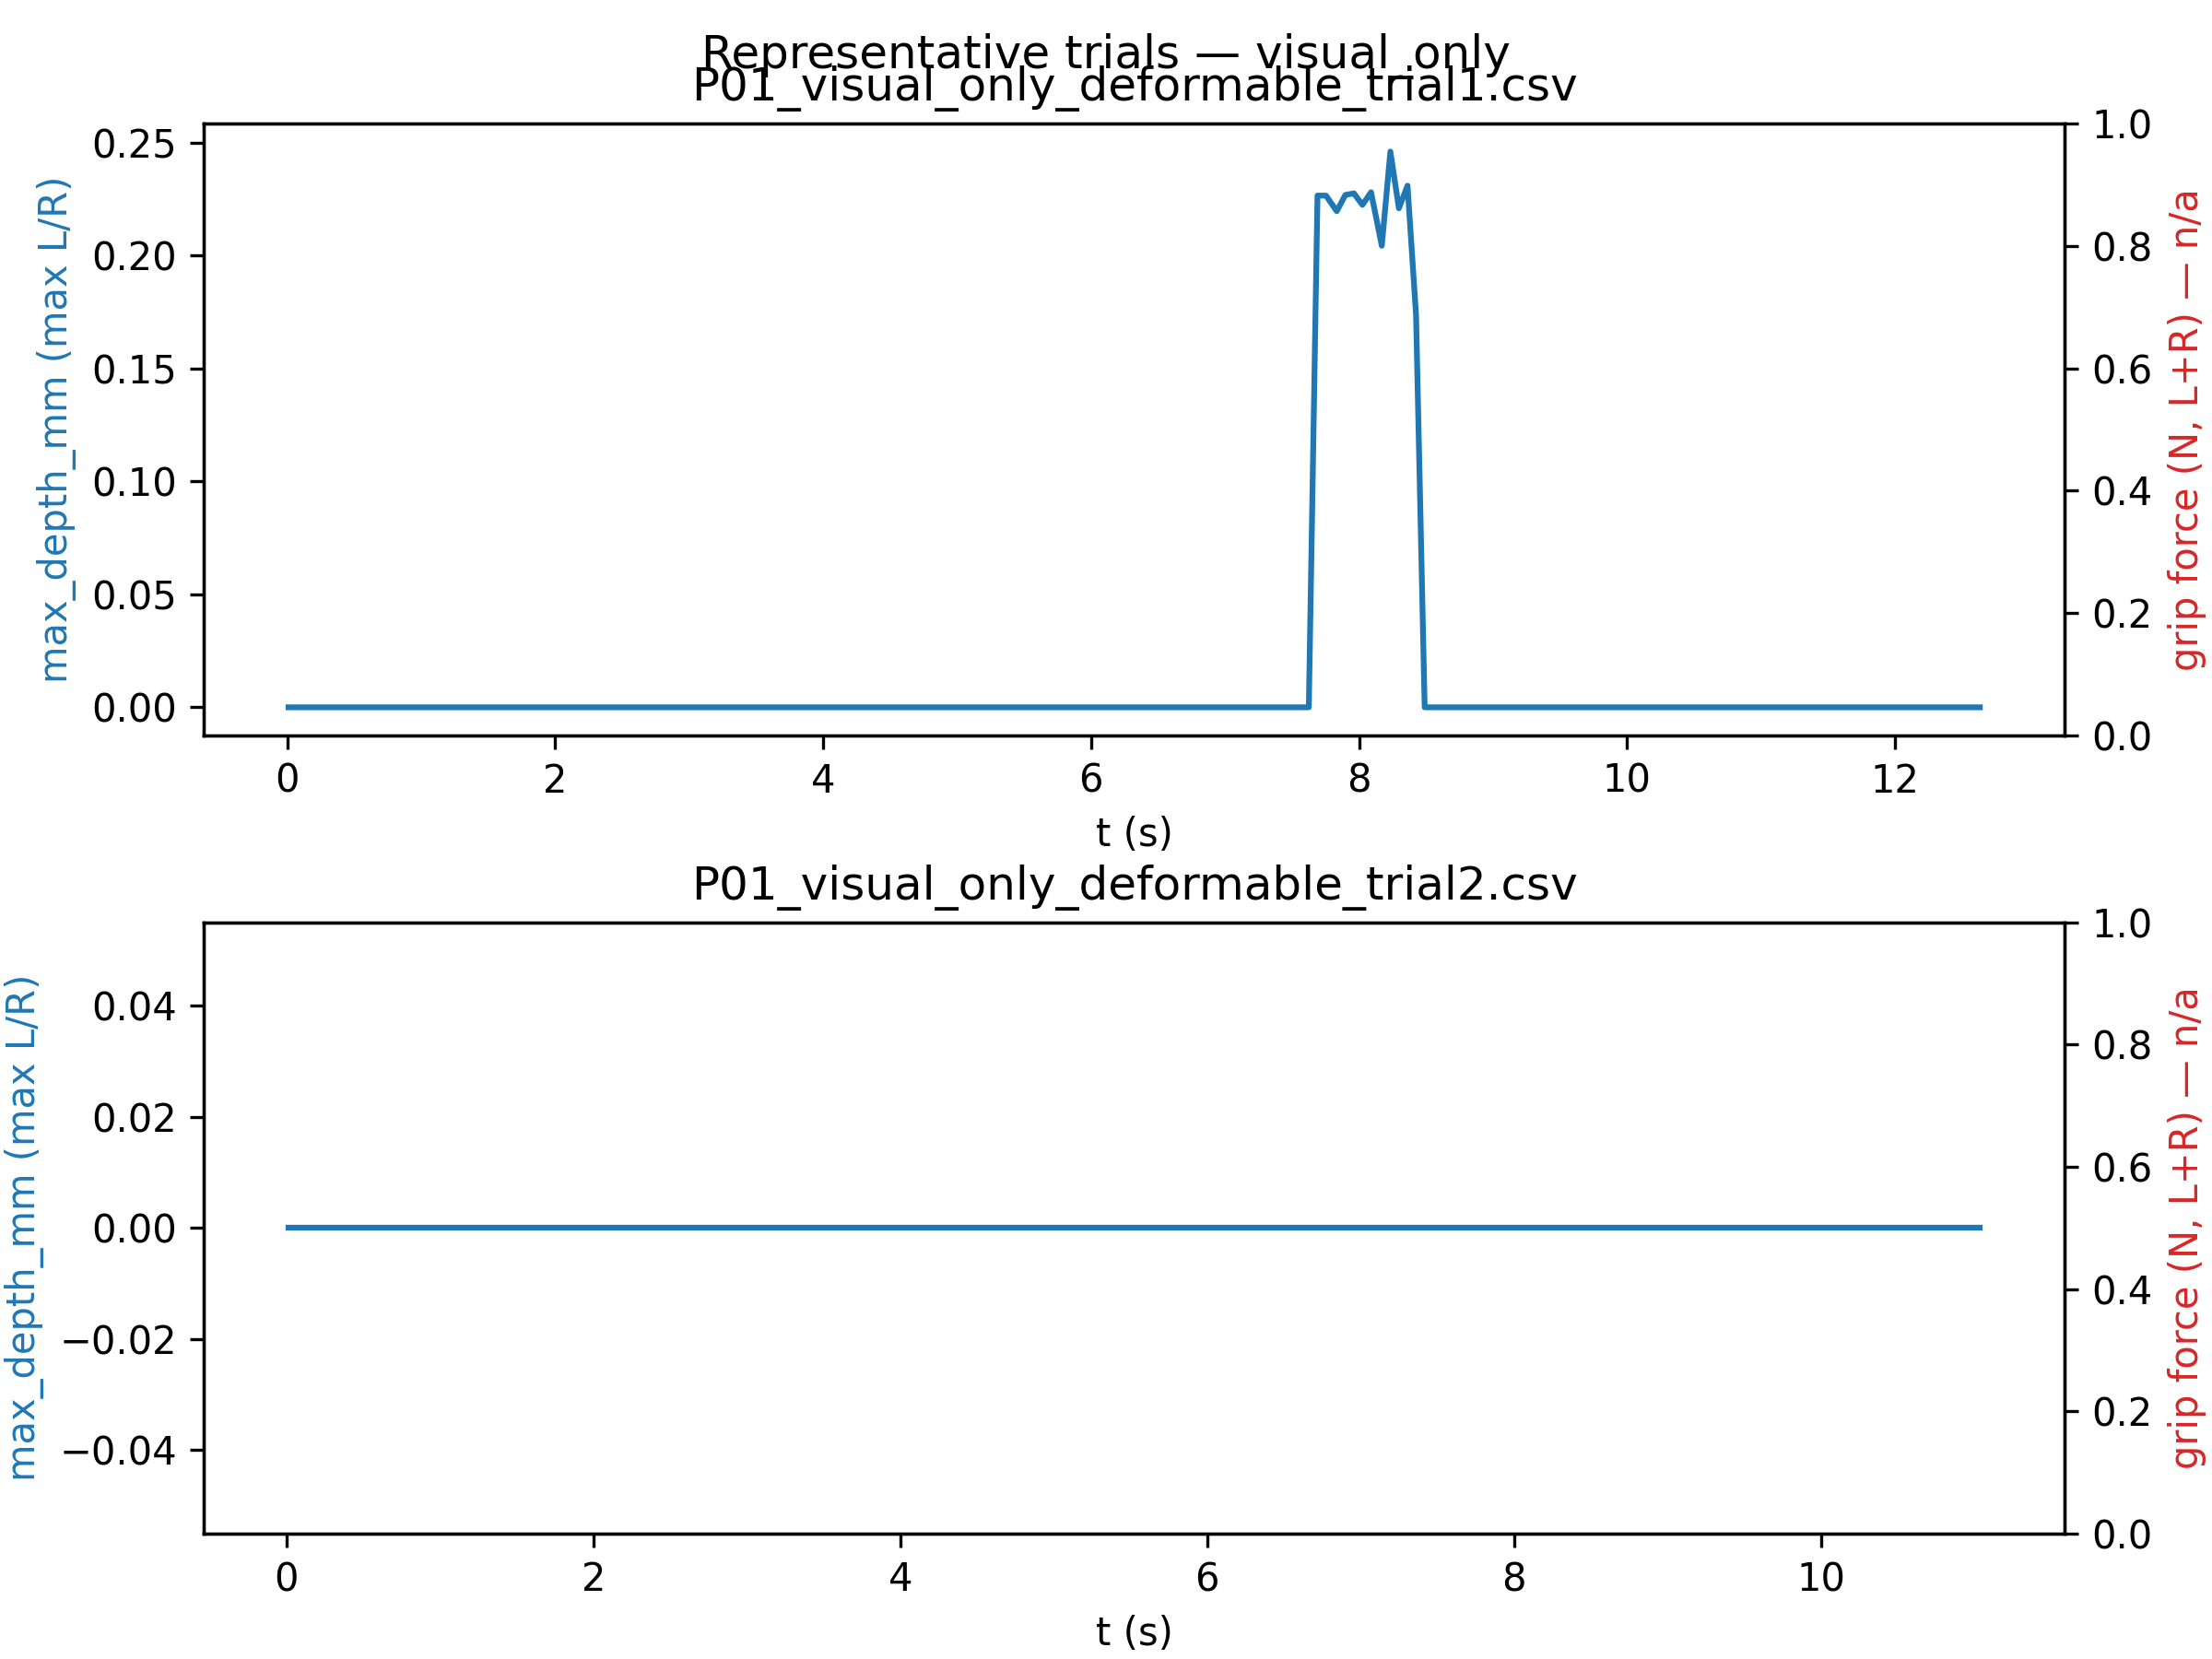
\includegraphics[width=\textwidth]{section_5_5_timeseries_visual_only.png}
        \caption{Visual-only}
    \end{subfigure}
    \hfill
    \begin{subfigure}[b]{0.48\textwidth}
        \centering
        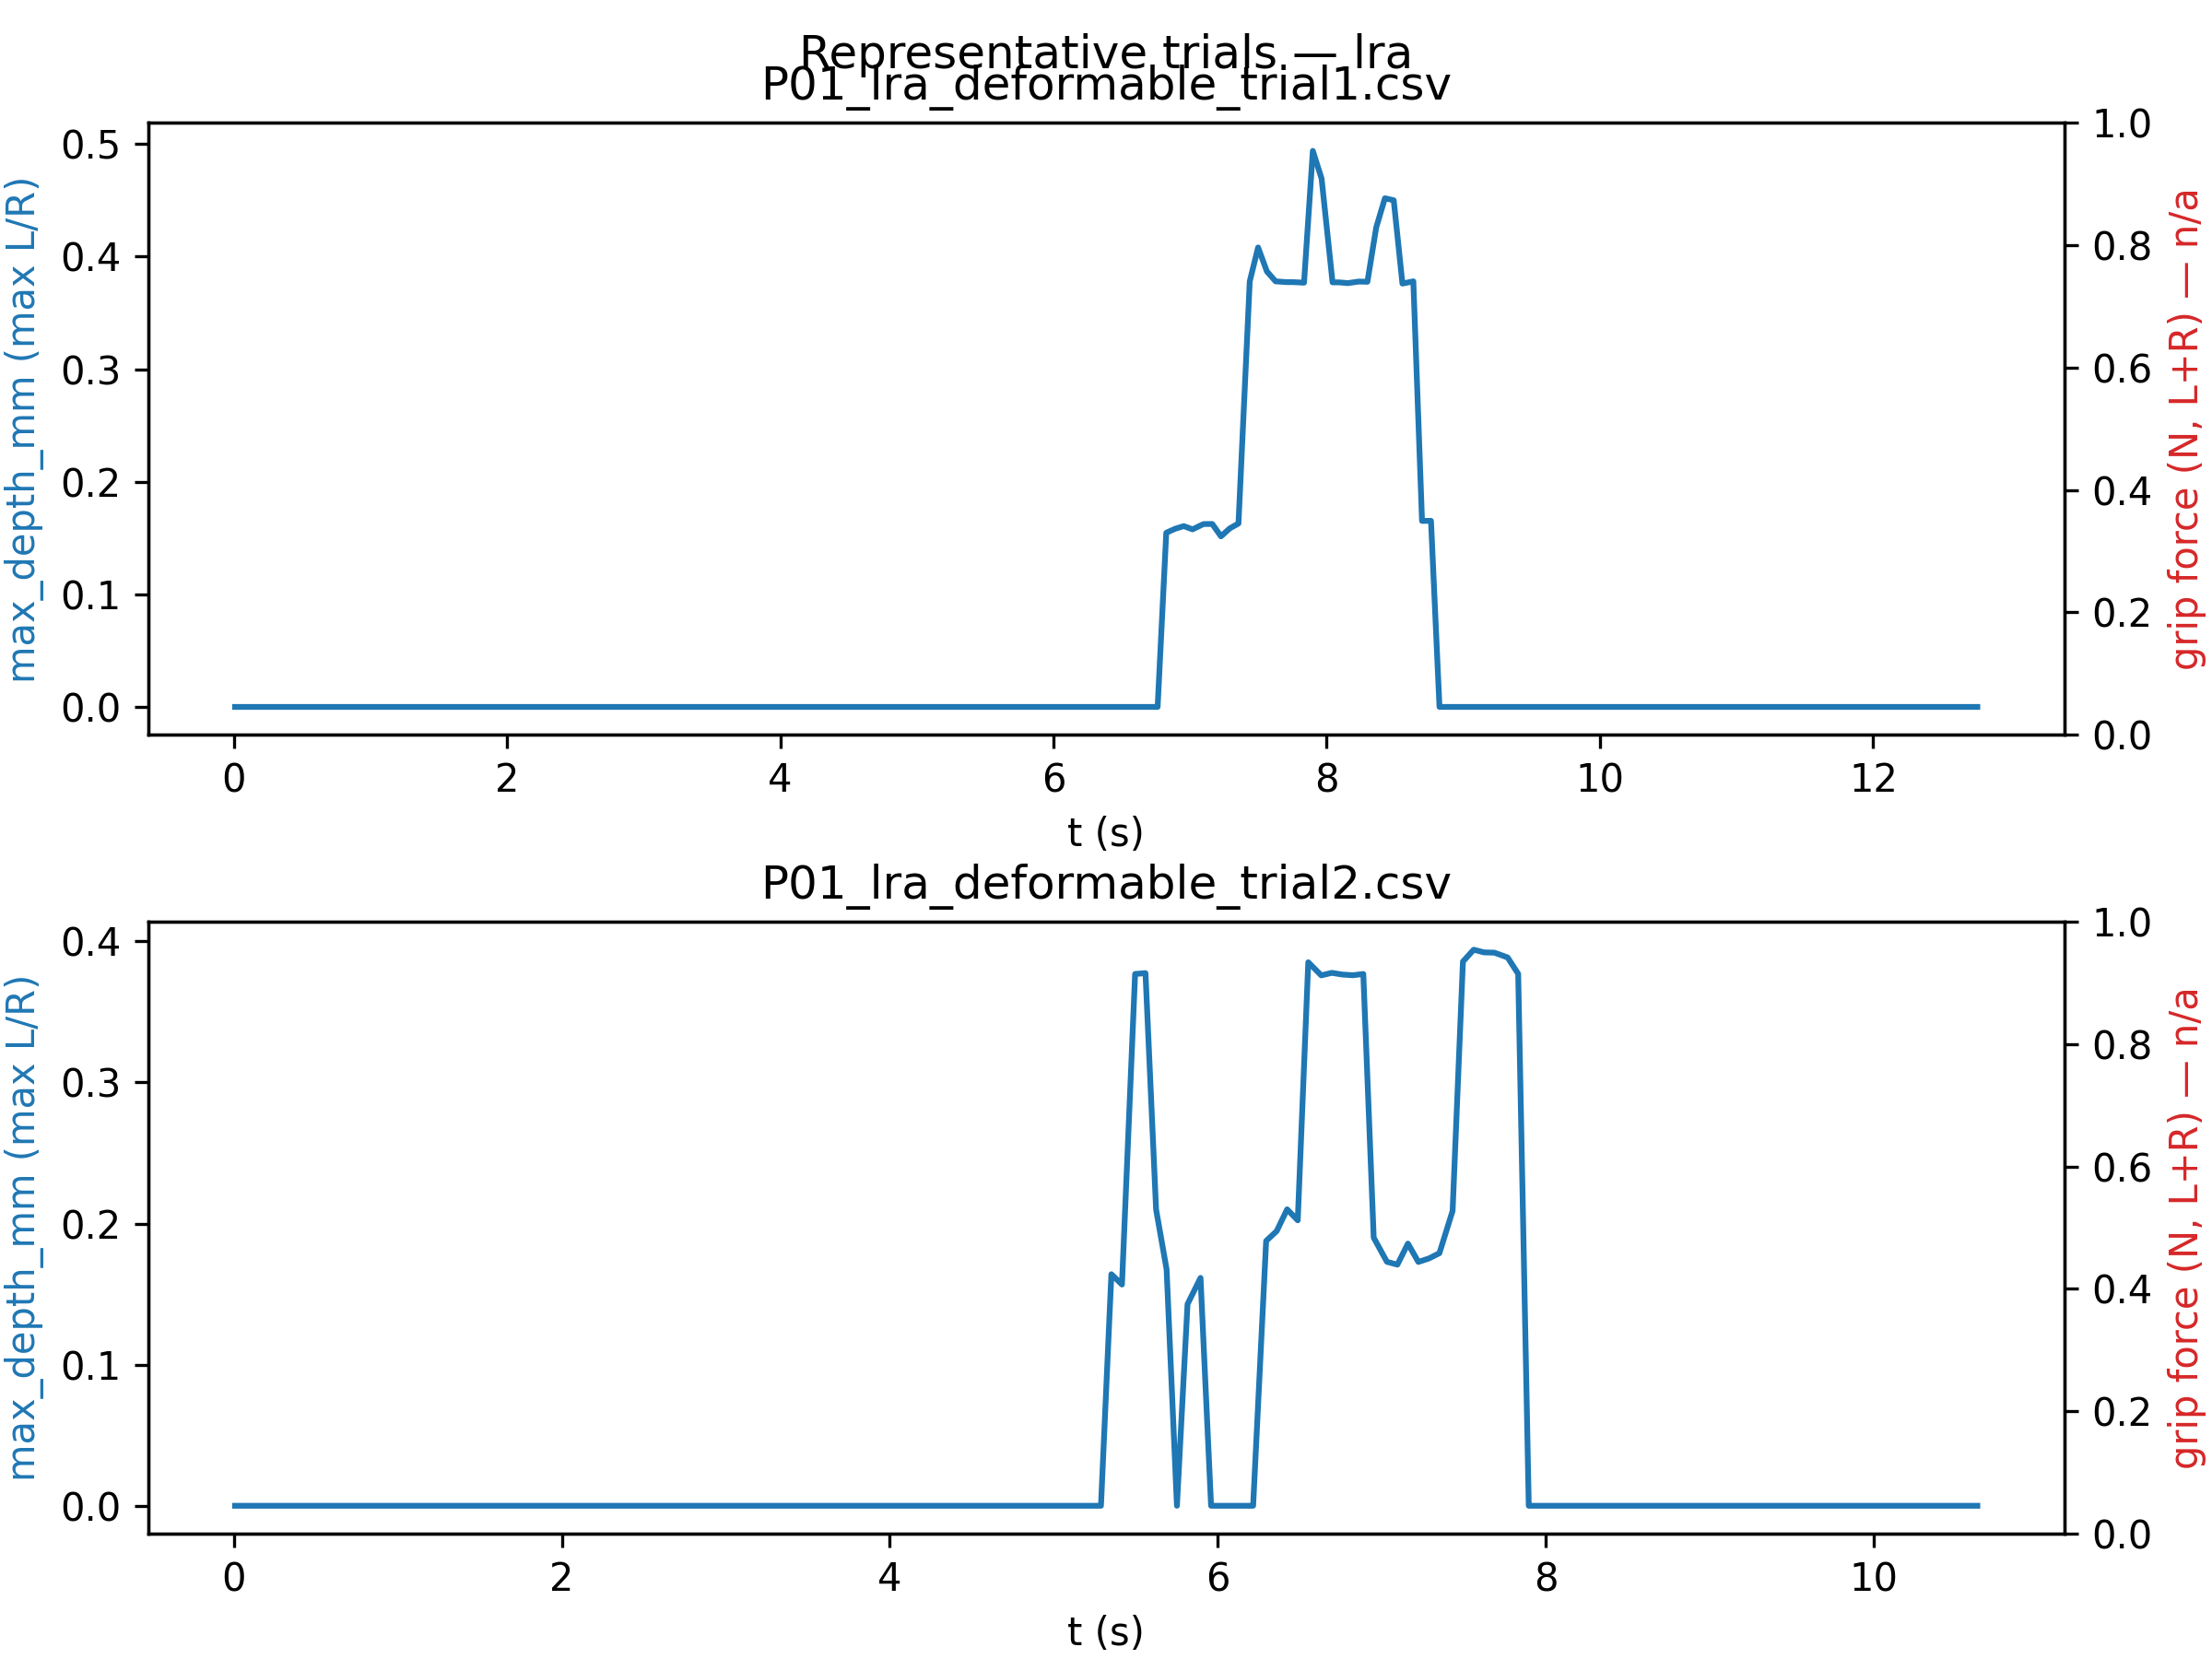
\includegraphics[width=\textwidth]{section_5_5_timeseries_lra.png}
        \caption{LRA}
    \end{subfigure}
    \\[1ex]
    \begin{subfigure}[b]{0.48\textwidth}
        \centering
        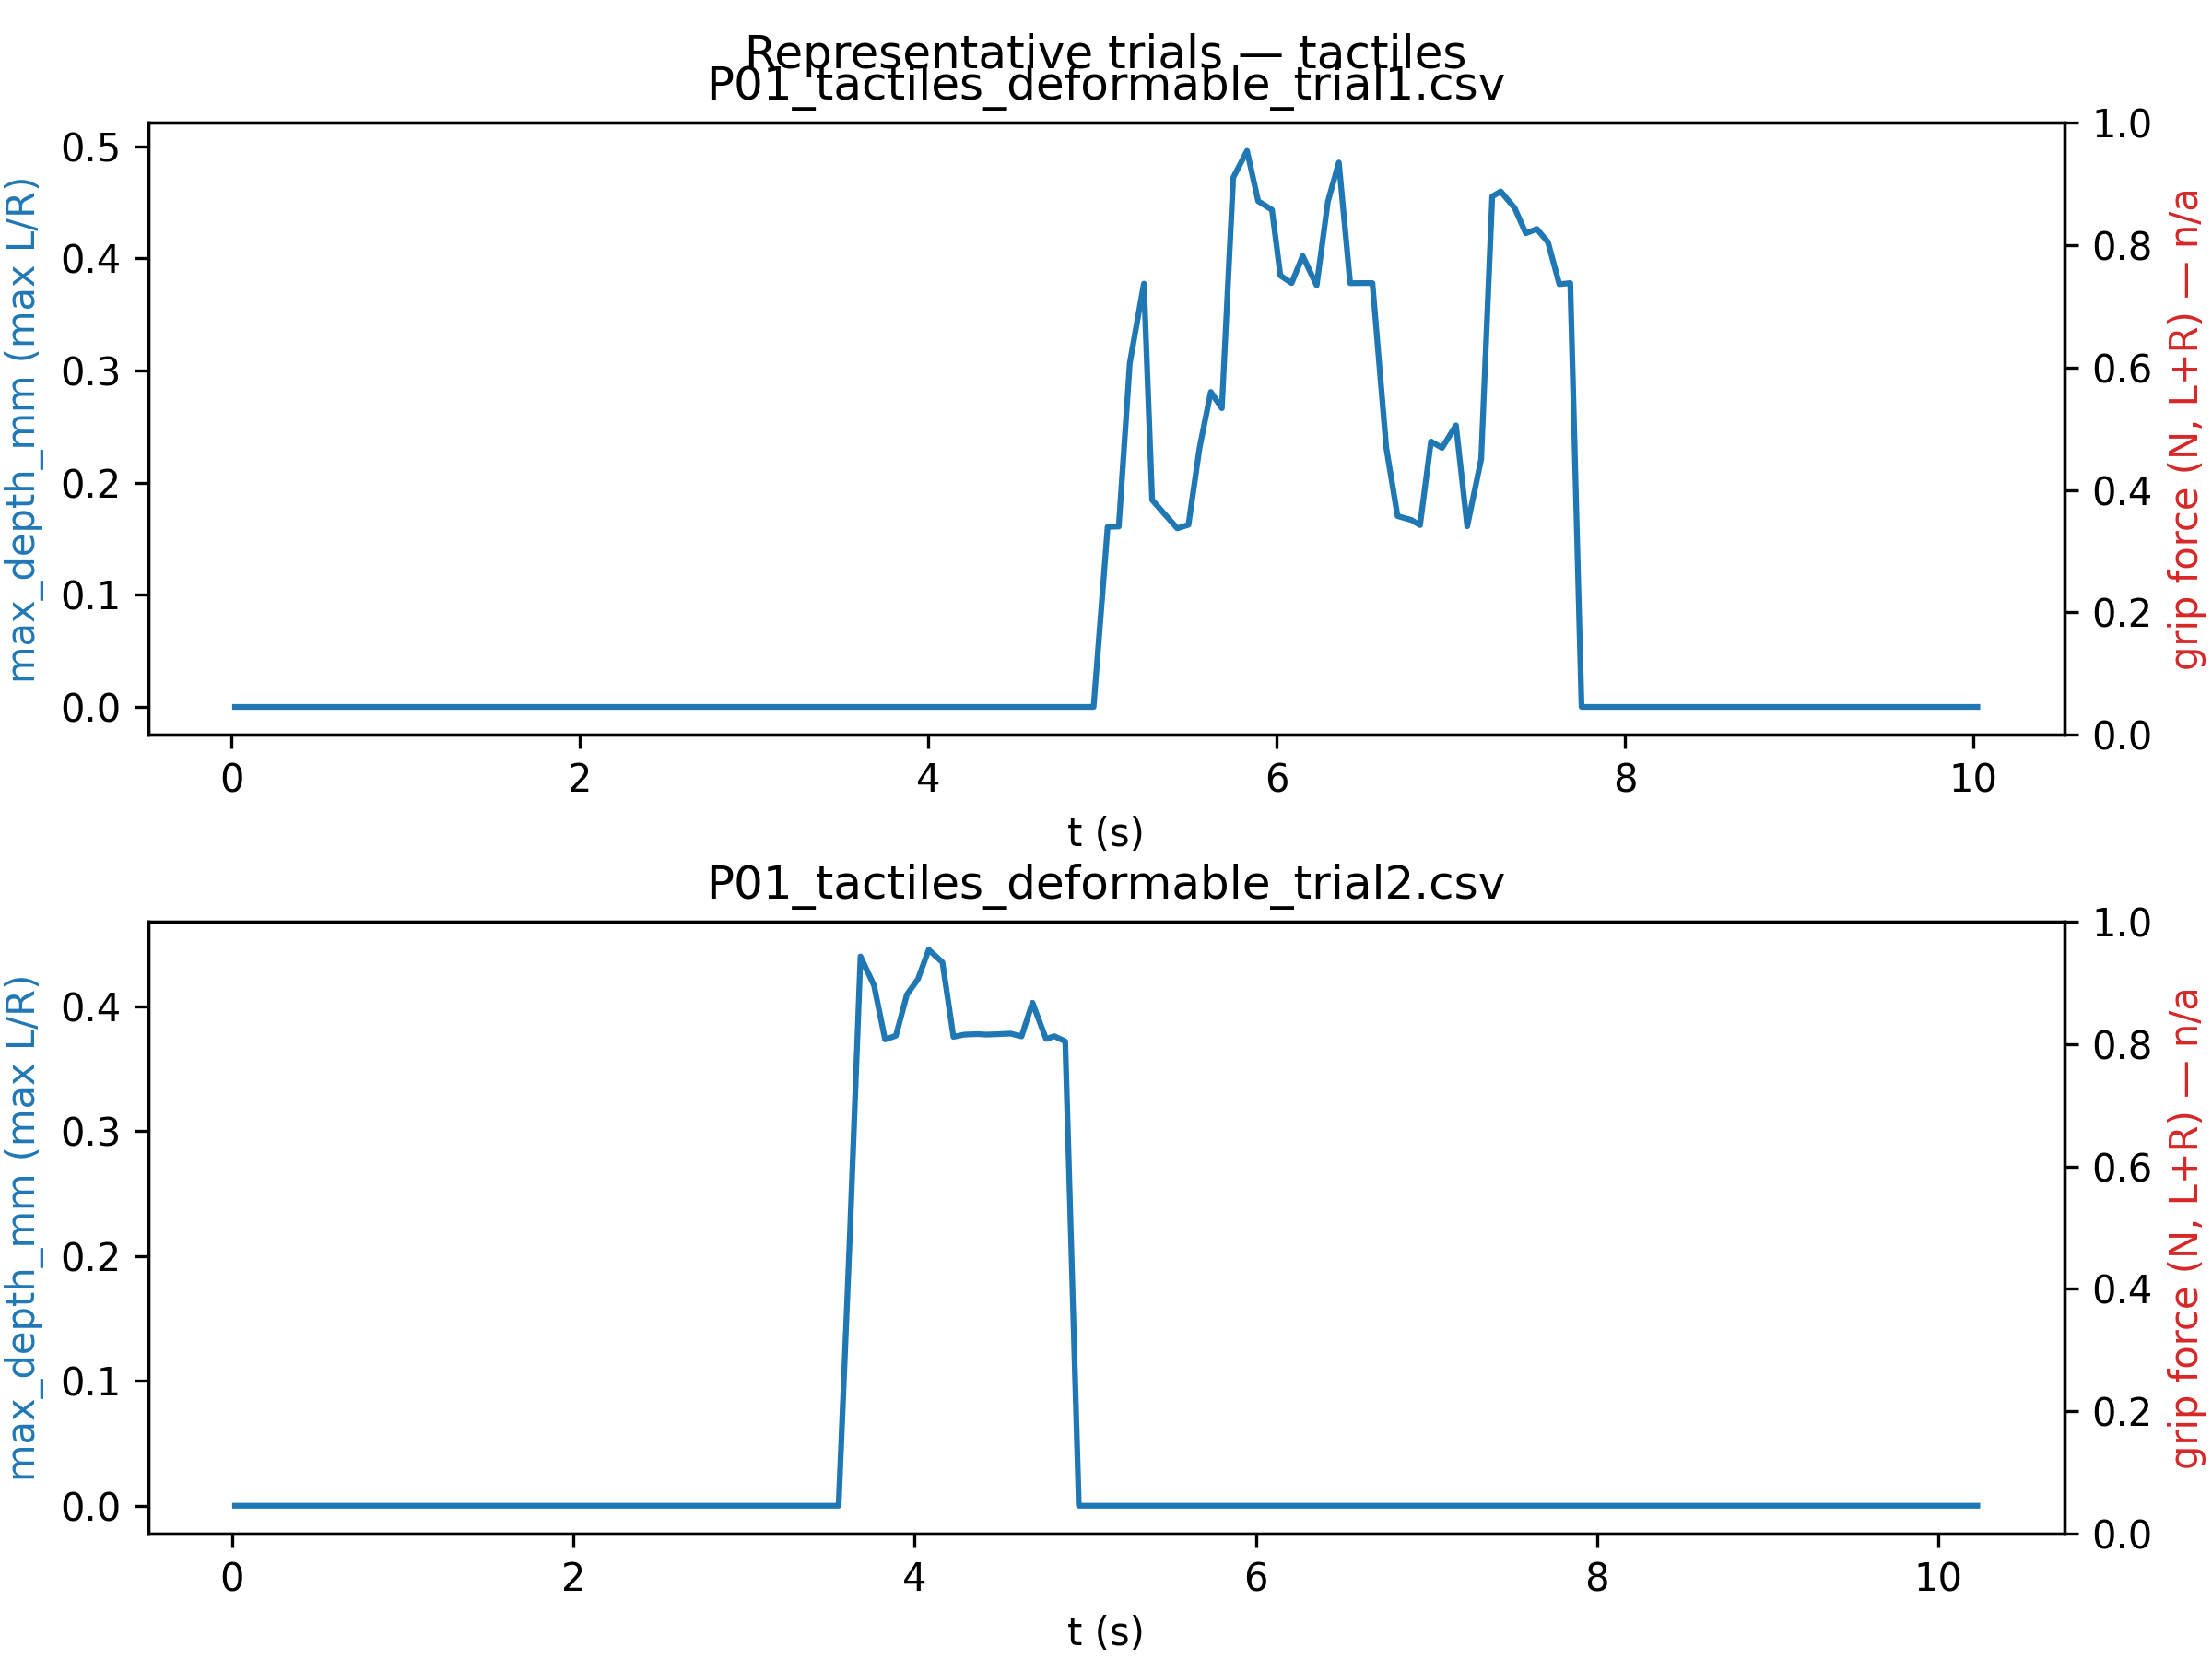
\includegraphics[width=\textwidth]{section_5_5_timeseries_em.png}
        \caption{EM}
    \end{subfigure}
    \caption{Representative single-trial traces of indentation depth and
        deformation volume against time, one per feedback condition.}
    \label{fig:timeseries}
\end{figure}

\section{Subjective Results}
\label{sec:results-likert}

Participants rated both haptic conditions above visual-only feedback, most
strongly on items concerning the ability to feel grip force and confidence in
the grasp (Figure~\ref{fig:likert}). In the forced-choice preference question
the LRA was the most frequently selected condition. No individual questionnaire
item separated the two haptic conditions reliably.

\begin{figure}[htbp]
    \centering
    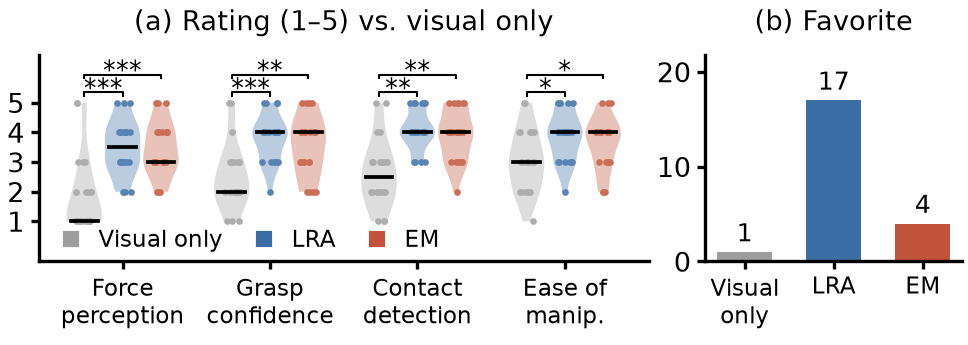
\includegraphics[width=0.9\textwidth]{preprint_fig6.png}
    \caption{Subjective results. (a) Item-by-item ratings relative to
        visual-only feedback, $N=22$; additional star marks indicate stronger
        statistical reliability. (b) Share of forced-choice favourite picks per
        condition.}
    \label{fig:likert}
\end{figure}

\todo{Insert the per-item medians and IQRs and the Friedman/Wilcoxon statistics
    from \texttt{section\_5\_6\_likert\_summary.csv} and
    \texttt{section\_5\_6\_likert\_friedman.csv}, and the preference counts from
    \texttt{section\_5\_6\_likert\_preference.csv}.}

% =====================================================================
\chapter{Discussion}
\label{ch:discussion}
% =====================================================================

\section{Interpretation}
\label{sec:interpretation}

The results separate cleanly into a strong effect and a weak one.

The strong effect is the presence of tactile feedback. For fragile objects, both
haptic conditions reduced excess deformation by roughly an order of magnitude
and raised survival by 16--19 percentage points over visual-only feedback. The
mechanism is visible in the time-series traces: under visual-only feedback the
operator has no signal that indicates when the useful part of the grasp is
complete, and continues to squeeze after contact is fully established. The
haptic conditions supply exactly that signal, and the metric most improved is
the one that measures effort applied after the signal saturates. That the effect
appears in survival, not merely in the force proxy, is what makes it
practically meaningful.

The weak effect is actuator type. The LRA produced the lower excess deformation
and was the more frequently preferred condition; the EM produced fewer grip
adjustments. Neither difference is large relative to between-participant spread,
and no questionnaire item distinguished the two. The honest reading is that this
study establishes that feedback helps, and does not establish which actuator
helps more.

The absence of any effect on deformable objects is not a failure of the system
but a property of the task. A foam cube imposes no penalty for over-squeezing,
so a channel whose value lies in discouraging over-squeezing has nothing to act
on. This asymmetry is itself informative: it suggests the benefit of tactile
feedback in teleoperation is concentrated in tasks with a failure threshold
rather than distributed across manipulation generally.

\section{Limitations}
\label{sec:limitations}

Several features of the study bound how strongly these conclusions can be
stated.

\paragraph{Condition order.} Conditions were presented in a fixed order rather
than counterbalanced across participants. Practice effects across the session
and fatigue toward its end are therefore confounded with condition, and a
difference attributed to an actuator may in part reflect its position in the
session.

\paragraph{The two actuators differ in more than one way.} They differ in
transduction mechanism, but also in placement on the hand and in how well hand
tracking performed while each was worn. A preference for one actuator may
therefore reflect smoother control rather than a better sensation.

\paragraph{Rendering narrows the intended contrast.} The intended contrast was
continuous versus discretely-switched rendering. In practice the LRA is driven
by envelope modulation of a fixed-amplitude carrier rather than by true
amplitude modulation (Section~\ref{subsec:lra-drive}), so both conditions set
intensity by gating a waveform on and off, differing chiefly in temporal
granularity. A dedicated resonant-driver IC capable of amplitude modulation
would sharpen the contrast.

\paragraph{Off-resonance carrier.} The LRA carrier was set empirically to
approximately \SI{200}{\hertz} rather than tuned to the measured resonance of
the specific actuators. Since an LRA is efficient only in a narrow band around
resonance, the achievable amplitude range, and therefore the perceptual dynamic
range of the intensity signal, may have been compressed.

\paragraph{Differing native temporal response.} The LRA requires several drive
cycles to ring up and ring down; the EM latch transitions almost instantly. A
comparison intended to isolate rendering style is therefore partly a comparison
of responsiveness.

\paragraph{Uncalibrated force.} Grip force is inferred from deformation volume
in arbitrary units, not measured in newtons, and indentation depth rests on a
single-ball calibration never checked against an independent gauge, so its
millimetre scale carries unquantified error.

\paragraph{Tracking and latency.} Hand tracking is 2D and uncalibrated, and the
end-to-end sensor-to-actuator latency still requires the bench measurement
described in Section~\ref{sec:latency}.

\section{Energy-Based Modelling of the Loop}
\label{sec:phs}

At an abstract level the system is an interconnection of energy-exchanging
subsystems: the gripper-object contact, the sensing and computation pipeline,
and the actuator-skin interface. Port-Hamiltonian systems theory models such
networks in terms of power-conjugate variables and has been used to establish
passivity and stability guarantees in bilateral teleoperation \cite{secchi2007}. A full
port-Hamiltonian treatment of this system, with the contact, the tactile
sensor's deformation measurement, and the EM actuator's stored magnetic energy
each modelled as a port, lies beyond the scope of this thesis, but would
offer a principled account of why one actuator class transmits sensed
deformation more transparently than another, grounded in the energetics of the
loop rather than in empirical comparison alone.

% =====================================================================
\chapter{Conclusion}
\label{ch:conclusion}
% =====================================================================

This thesis presented an end-to-end tactile-haptic teleoperation system that
integrates vision-based tactile sensing into a Robotiq 2F-85 adaptive gripper,
commands the gripper from the operator's own pinch aperture, and renders the
sensed contact deformation on a five-channel wearable actuator array through
either linear resonant actuators or electromagnetic bistable pin actuators,
with an identical sensing and intensity-mapping pipeline upstream of the driver
in both cases.

A within-subjects study with $N=22$ participants found that tactile feedback
made the grasping of fragile objects substantially safer: excess deformation
(force applied after the tactile display had saturated) fell by close to
an order of magnitude, and object survival rose from 62\% under visual-only
feedback to 81\% with the LRA and 78\% with the EM. Deformable objects, which
lack a failure threshold, showed no reliable effect. Participants preferred both
haptic conditions to visual-only feedback and most often chose the LRA, but no
questionnaire item separated the two actuators reliably.

The conclusion is therefore asymmetric, and deliberately so: the presence of
tactile feedback matters, and the choice between these two actuators, under
these conditions and at this sample size, does not demonstrably matter. Ranking
actuator types would require a study that removes the confounds identified in
Section~\ref{sec:limitations}: counterbalanced condition order, matched
placement on the hand, resonance-tuned amplitude-modulated LRA drive, and a
force proxy calibrated in newtons.

Future work follows directly from these limitations, and from one extension the
present system does not exploit: the tactile sensor produces a full depth map,
of which this study renders a single scalar per finger. Rendering the spatial
structure of the contact patch across the actuator array, rather than
collapsing it to one intensity, is the most promising direction for
recovering more of the information the sensor already measures.

% =====================================================================
%  BACK MATTER
% =====================================================================
\cleardoublepage
\begingroup
\raggedright
\printbibliography[heading=bibintoc, title={References}]
\endgroup

\appendix
\cleardoublepage

\chapter{Questionnaire Items}
\label{app:questionnaire}
\todo{Reproduce the questionnaire exactly as administered, including the
    demographic and screening items and the closing preference question.}

\chapter{Per-Participant Summary Data}
\label{app:data}
\todo{Table of per-participant, per-condition medians for each metric of
    Section~\ref{sec:metrics}, generated from
    \texttt{section\_5\_1\_reduced\_metrics.csv}.}

\chapter{Firmware and Driver Details}
\label{app:firmware}
\todo{Driver schematic, bill of materials, pulse-timing parameters, and the
    serial packet format used between host and ESP32-C6.}

\cleardoublepage
\chapter*{Acknowledgements}
\addcontentsline{toc}{chapter}{Acknowledgements}
\todo{Acknowledge \supervisorname, the laboratory, and the study participants.}

\end{document}
